\documentclass{beamer}

\title{Matrix Project}
\subtitle{\\Ashutosh Tiwari - CS18BTECH11049 \\ Polamraju Aakarsh - ES18BTECH11027}

%\usetheme{lucid}
\begin{document}
	\frame {
		\titlepage
	}
	%page 2
	\frame {
		\frametitle{Question in Geometry :-}
	    Let P be a point on the parabola \[x^2+4y=0\] Given that the 				distance of P from the centre of the circle \[x^2+y^2+6x+8=0\] 				is minimum. Find the equation of the tangent to the parabola at 			P.
	}
	%page 3
	\frame {
		\frametitle{Question in Matrix :-}
	    Let P be a point on the parabola \\ \hspace{3cm} x^{T}						\begin{bmatrix}
	    1 & 0\\
	    0 & 0
	    \end{bmatrix}x + \begin{bmatrix}
	    0 & 4
	    \end{bmatrix} x = 0 . \\Given that the distance of P from the centre 				of the circle \\ \hspace{3cm} x^{T}x + \begin{bmatrix}
	    6\\
	    0 
	    \end{bmatrix}x + 8 = 0\\is minimum. Find the equation of the 					tangent to the parabola at P.
	}
	
%Questions written till here.
	%page 4
	\frame {
		\frametitle{Solution :-}
	    \hspace{1cm} Equation of parabola is : x^{T}Vx + 2U^{T}x + F =0 \\ \hspace{1cm} Equation of circle is : x^{T}x + 2C_{p}^{T}x + E =0\\ \ here V = \begin{bmatrix}
	    1 & 0\\
	    0 & 0
	    \end{bmatrix}, U = \begin{bmatrix}
	    0 \\
	    2 
	    \end{bmatrix}, C_{p} = \begin{bmatrix}
	    6 \\
	    0 
	    \end{bmatrix}, F = 0 and E = 8.\\ Let C be the centre of circle, r be the radius of the circle and x_{1} be any point on the given circle.\\ \implies \hspace{1cm} (x_{1} - C)^{T}(x_{1}-C) = r^{2}\\ 
\implies \hspace{1cm} x_{1}x_{1}^{T} - 2C^{T}x + CC^{T} - r^{2} = 0.\\
Comparing this equation with the equation of circle:\\ \hspace{1.5cm} -2C^{T}=C_{p}^{T}\\ \implies \hspace{1cm} C = \frac{-1}{2} C_{p} = \begin{bmatrix}
	    -3 \\
	    0 
	    \end{bmatrix}
	}
	%page 5
	\frame {
		\frametitle{Solution continued..}
		The equation of a tangent to given parabola at any point P on the parabola is :\\ \hspace{1.5cm} (P^{T}V + U^{T})x + P^{T}U	+ F = 0.\\ \implies \hspace{1cm} (P^{T}V + U^{T})x = -P^{T}U - F \\ Comparing with the equation of line : n^{T}x = \lambda \\ \hspace{1.5cm} n^{T} = P^{T}V = U^{T}\\ \implies \hspace{1cm} n = (P^{T}V + U^{T})^{T} = PV^{T} + U\\ Since P lies on the line n^{T}x= \lambda \\ \implies \hspace{1cm} n^{T}P = \lambda \\ Then equation of the tangent can be rewritten as \\ \hspace{1cm} n^{T}x = n^{T}P  \implies  n^{T}(x-P) = 0 
	}	
	%page 6
	\frame {
		\frametitle{Solution Approch :}
		For P to be the point on parabola whose distance is minimun from centre of the circle, \textbf{CP} must be normal to the parabola.\\ \implies \\ \hspace{2cm} \textbf{CP}  is perpendicular to tangent 
}
		%page7
		\frame {
		\frametitle{Solution continued..}
		 \hspace{2cm} \textbf{CP}  is perpendicular to tangent	\\ \implies \textbf{CP} \perp \textbf{xP}, where \hspace{.05cm} x \hspace{.05cm} is \hspace{.05cm} any \hspace{.05cm} point \hspace{.05cm} on \hspace{.05cm} the \hspace{.05cm} tangent \hspace{.05cm} to \hspace{.05cm} the \hspace{.05cm} \\ \hspace{2cm} parabola \hspace{.05cm} at \hspace{.05cm} P\\ 
\implies \hspace{1cm} (C-P)^{T}(x-P) = 0\\ \hspace{1cm} Since (C-P)^{T}(x-P) = 0\hspace{0.5cm} and \hspace{0.5cm} n^{T}(x-P) = 0 \\ \implies \hspace{1cm} n = k(C-P), where \hspace{.05cm} is \hspace{.05cm} a \hspace{.05cm} scaler. \\ \implies \hspace{1cm} n = K(C-P) \\ \hspace{6cm} Here K = \begin{bmatrix}
	    k & 0\\
	    0 & k
	    \end{bmatrix} \\ \implies \hspace{1cm} PV^{T} + U = KC - KP \hspace{1cm} \{n =  PV^{T} + U\} \\ \implies \hspace{1cm} P(V^{T}+K) = KC - U \\ \implies \hspace{1cm} P = (KC -U) (V^{T}+K)^{-1} 
	}
	%page 8
	\frame {
		\frametitle{Solution continued..}
		\\ \implies \hspace{0.25cm} P = \Bigg( \Bigg( \begin{bmatrix}
	    k & 0\\
	    0 & k
	    \end{bmatrix} \begin{bmatrix}
	    -3\\
	    0
	    \end{bmatrix} \Bigg) - \begin{bmatrix}
	    0\\
	    2
	    \end{bmatrix} \Bigg) \Bigg( \begin{bmatrix}
	    1 & 0\\
	    0 & 0
	    \end{bmatrix} + \begin{bmatrix}
	    k & 0\\
	    0 & k
	    \end{bmatrix}\Bigg)^{-1} \\ On solving, we get \\ \\
	    P = \hspace{1cm} \left[\begin{matrix}
    \frac{-3k}{k+1}  \\[6pt]
    \frac{-2}{k}
    \end{matrix}\right] \\ 
Since P lies on the parabola, sbstituting P in the equation of parabola : \\ 	\hspace{2cm} x^{T}Vx + 2U^{T}x + F =0 \\
\hspace{1cm} we get   P^{T}VP + 2U^{T}P + F =0 \\
 \implies \hspace{0.5} \Bigg( \left[\begin{matrix}
    \frac{-3k}{k+1}  & \frac{-2}{k}\\[6pt]
    \end{matrix}\right] \begin{bmatrix}
	    1 & 0\\
	    0 & 0
	    \end{bmatrix} \left[\begin{matrix}
    \frac{-3k}{k+1}  \\[6pt]
    \frac{-2}{k}
    \end{matrix}\right]  \Bigg) + \Bigg( \begin{bmatrix}
	    0 & 4\\
	    \end{bmatrix} \left[\begin{matrix}
    \frac{-3k}{k+1}  \\[6pt]
    \frac{-2}{k}
    \end{matrix}\right] \Bigg)  + 0 = 0\\
		}
		%page 9
		\frame {
		\frametitle{Solution continued..}
		solving, we get: \left[\begin{matrix}
    \frac{-3k}{k+1}  \\[6pt]
    \end{matrix}\right]  ^{2} + \left[\begin{matrix}
    \frac{-8}{k}  \\[6pt]
    \end{matrix}\right]  = 0
    \\.\\ \hspace{2cm}\left[\begin{matrix}
    \frac{9k^{2}}{k^{2}+2k+1}  \\[6pt]
    \end{matrix}\right] = \left[\begin{matrix}
    \frac{8}{k}  \\[6pt]
    \end{matrix}\right]
    \\.\\ \hspace{2cm}9k^{3} - 8k^{2} - 16k - 8 = 0\\.\\ \hspace{2cm}(k-2)(9k^{2}+10k+4)=0\\.\\ \hspace{2cm} k = 2
		}
		%page 10
		\frame {
		\frametitle{Solution continued..}
		\hspace{1cm}  P = \left[\begin{matrix}
    \frac{-3k}{k+1}  \\[6pt]
    \frac{-2}{k}
    \end{matrix}\right] , substituting \hspace{1cm} k=2 \\ \hspace{1cm} P =  \left[\begin{matrix}
    -2  \\[6pt]
    -1
    \end{matrix}\right] \\ The equation of a tangent to given parabola at any point P on the parabola is :\\ \hspace{1.5cm} (P^{T}V + U^{T})x + P^{T}U	+ F = 0. \\ substituting  \hspace{1cm} P =  \left[\begin{matrix}
    -2  \\[6pt]
    -1
    \end{matrix}\right] \\	
    \hspace{0.5cm} \Bigg( \begin{bmatrix}
	    -2 & -1\\
	    \end{bmatrix}\begin{bmatrix}
	    1 & 0\\
	    0 & 0
	    \end{bmatrix} + \begin{bmatrix}
	    0 & 2  \\
	    \end{bmatrix} \Bigg) x + \begin{bmatrix}
	    -2 & -1\\
	    \end{bmatrix} \begin{bmatrix}
	    0\\
	    2
	    \end{bmatrix} = 0 \\ \implies \hspace{1cm} \begin{bmatrix}
	    -2 & 2 \\
	    \end{bmatrix} x -2 = 0 \\ \implies \hspace{1cm} \begin{bmatrix}
	    -1 & 1 \\
	    \end{bmatrix} x = 1
		}
		\frame {
		\frametitle{Answer :}
		The equation of the desired tangent is :-\\ . \\
		\hspace{2cm} \begin{bmatrix}
	    -1 & 1 \\
	    \end{bmatrix} x = 1
		}
		\frame {
		\frametitle{Graphical Verification}
		Plotting the tangent and the normal to this tangent at P, we graphically verify that the normal passes through the center of the circle and hence that P is thepoint on the parabola that is at minimum distance from the center of the circle. 
		}
		\frame {
		\frametitle{Graph}
		\begin{figure}
			\centering
			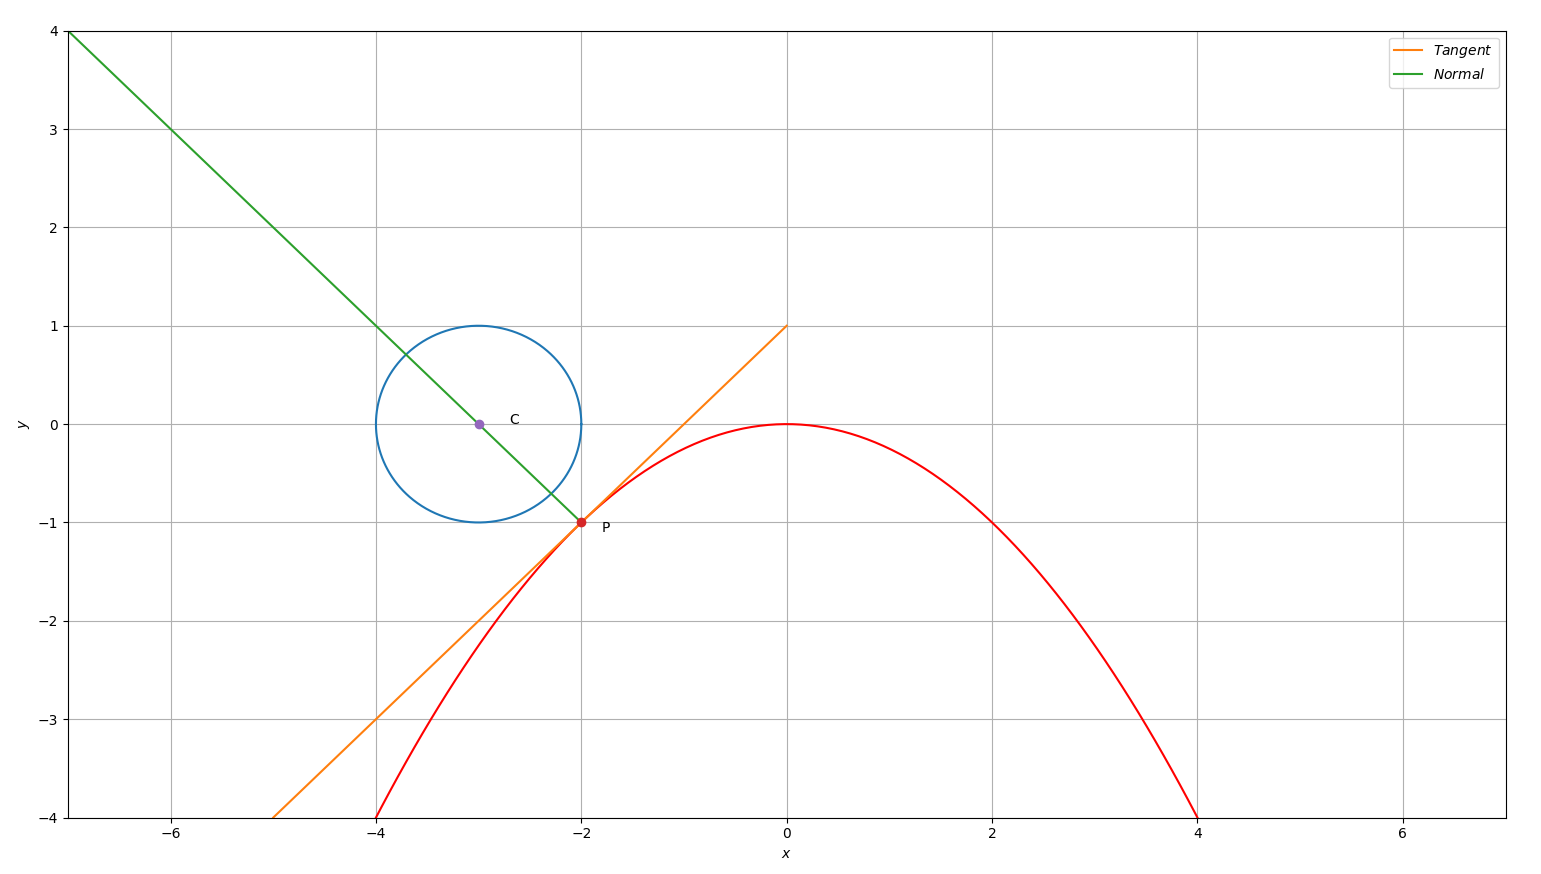
\includegraphics[scale=0.21]{figure2.png}
			\end{figure}
		}
\end{document}